\subsection{Models}
\mysubsubsection{Sandra Beuck}{Charaktere}

Innerhalb der Spielwelt gibt es vier modellierte Charaktere, welche in Cinema4D modelliert und animiert wurden. Unter zu Hilfenahme von Modeling- und Sculpting-Tools wurden liebevoll Details in die Figuren eingearbeitet. Aus zeitgründen wurden alle Modelle aus einem Grundmesh erstellt, ebenso die Bone-Animation. Im gesamten Spiel gibt es vier Charaktere, dies ist jedoch nur die prototypische Darstellung der Dorfbewohner. Im richtigen Spiel wären mehr und verschiedene Charaktere unterwegs. 

\mysubsubsection{Sandra Beuck}{Tiere}

\begin{figure}[!htbp]%[htbp]
	\centering
		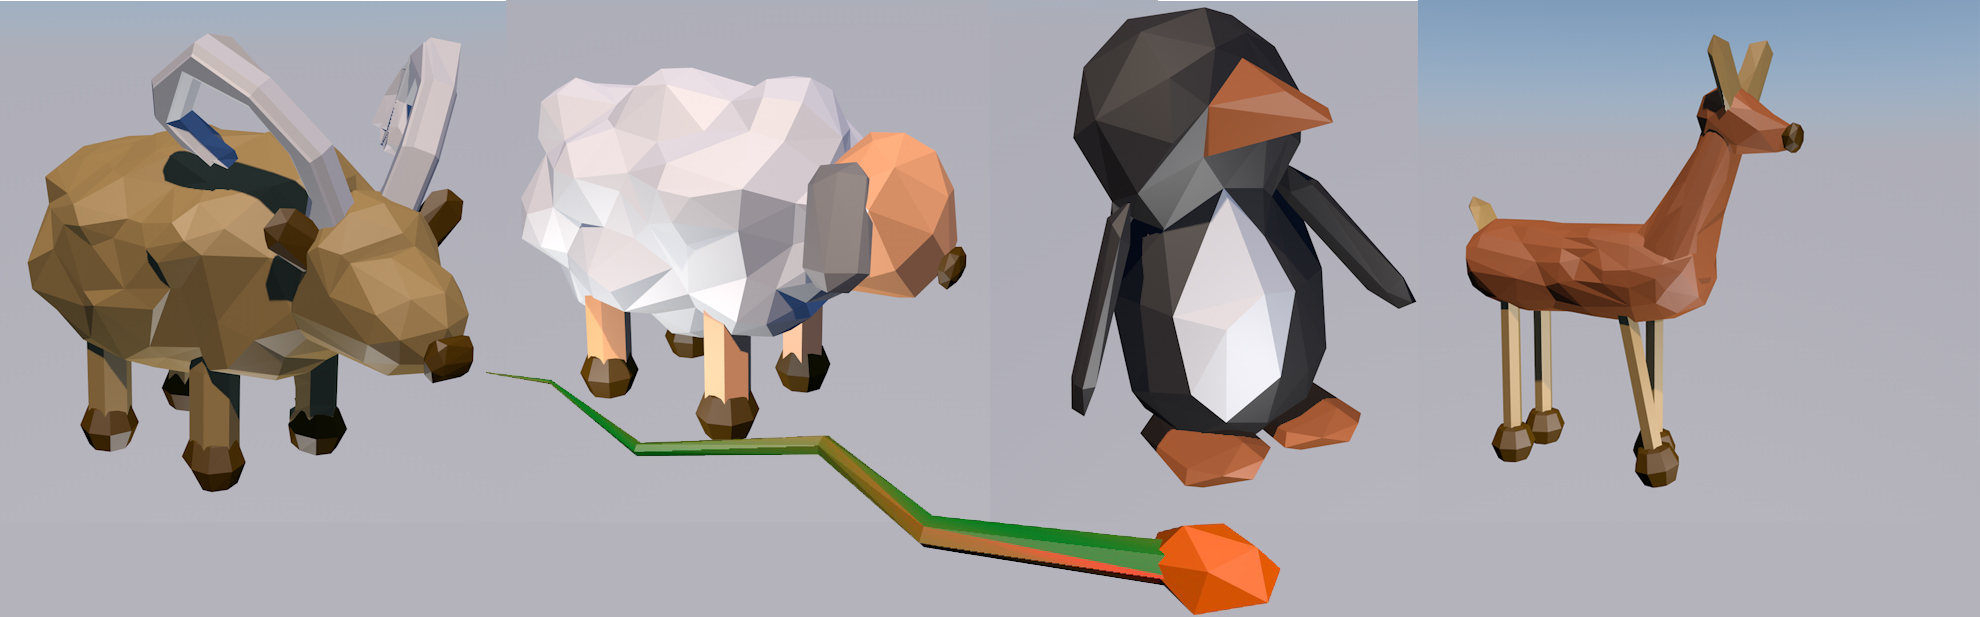
\includegraphics[width=1.0\textwidth]{images/tiere}
	\caption{Tiere}
	\label{fig:Tiere}
\end{figure}

Alle Tiere im Spiel sind animiert und mit Bones ausgestattet. Pro Welt gibt es ein charakteristisches Tier. Die Animation der Tiere wirkt dem Low-Poly-Look entsprechend etwas gröber, verleiht dem Spiel jedoch einen gewissen Charme. Um die Animation optimal abzubilden, haben die Tiere etwas mehr Polygone. 



\mysubsubsection{Sandra Beuck}{Gravitationsmaschine}

\begin{figure}[!htbp]%[htbp]
	\centering
		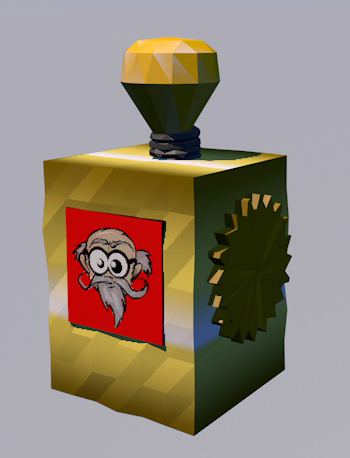
\includegraphics[width=0.6\textwidth]{images/gravinator}
	\caption{Gravitationsmaschine}
	\label{fig:gravinator}
\end{figure}

Die Gravitationsmaschine dient als Verbindungselement der Welten und ist in der Gebirgswelt prototypisch umgesetzt.

Sie ist eines der wichtigsten Elemente im Spiel, da sie in jeder Welt existent ist und somit ein Bezugspunkt für den Spieler darstellt. Aus diesem Grund ist die Gravitationsmaschine mit vielen Details, wie zum Beispiel einem Zahnrad, einem Bild des Wissenschaftlers und einer Kontrollleuchte versehen, und  erzeugt dadurch einen hohen Wiedererkennungswert. 

\mysubsubsection{Lydia Friedrich}{Remote Cube - Würfel}

\begin{figure}[!htbp]%[htbp]
	\centering
		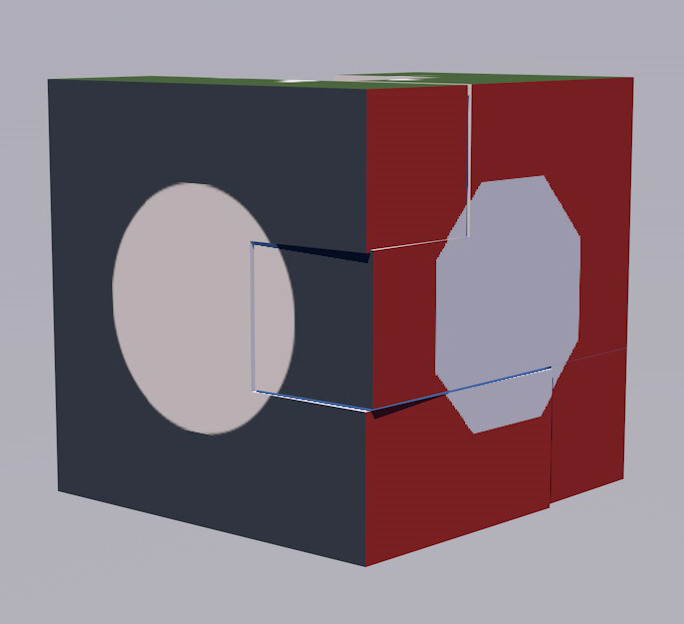
\includegraphics[width=0.6\textwidth]{images/RemoteCubeC4D}
	\caption{Virtueller Remote Cube}
	\label{fig:RemoteCube}
\end{figure}

Der Remote Cube ist die Verknüpfung des Würfels zur Außenwelt, denn nur mit ihm kann der Spieler das Spiel beenden und wieder in die reale Welt zurückkehren. Bevor dieses Ziel jedoch erreicht wird, müssen zunächst alle drei Teile des Remote Cubes erfolgreich vom Spieler eingesammelt werden (da der Remot Cube zu Beginn des Spiels zerbricht). Somit ist der Reomte Cube ebenfalls ein sehr wichtiges Spielelement, da er das Symbol für den erfolgreichen Abschluss des Spiels darstellt.

Er ähnelt optisch dem Markerwürfel den der Spieler während des Spielens in den Händen hält und schafft so einen Bezug zwischen virtueller und realer Welt. Mit Hilfe von UV Mapping werden die Symbole des Markerwürfels auf den Remot Cube übertragen.